 
\documentclass[a4paper]{article}
\usepackage[margin=2cm]{geometry}
\usepackage{graphicx}
\usepackage{enumitem}
\setlist[description]{}
\usepackage{hyperref}
\usepackage{fancyhdr}
\usepackage[utf8]{inputenc}

\hypersetup{
  colorlinks=true,
  linkcolor=black,
  urlcolor=blue,
  linktoc=all
}

\title{Torneos de Yu-Gi-Oh! \\
		Equipo 2
}
\author{
  \begin{tabular}{c}
    Chavely Gonz\'alez Acosta C312 \\
    Jos\'e Carlos Pendas Rodrigu\'ez C311 \\
    L\'azaro David Alba Ajete C311 \\
    Max Bengochea Mor\'e C311
  \end{tabular}
}
\date{\today}

\begin{document}
\pagenumbering{gobble}
\maketitle
\newpage

\clearpage
\pagenumbering{arabic}

\tableofcontents
\newpage

\section{Introducci\'on}

\subsection{Alcance del producto}
\subsection*{Descripci\'on del Producto}
Este sistema permitirá a los organizadores de torneos crear, administrar y seguir el progreso de torneos de Yu-Gi-Oh!, así como proporcionar a los jugadores una plataforma para registrarse en estos eventos y consultar estadísticas relevantes.

\subsection*{Límites del Producto}
El sistema de gestión de torneos de Yu-Gi-Oh! se centrará en la creación, administración y en el seguimiento de torneos de este juego de cartas. No incluirá características relacionadas con la venta de cartas ni con la implementación de las reglas del juego.

\subsection*{Dependencias y Suposiciones}
Una de las principales dependencias de este proyecto es la disponibilidad de servidores web y bases de datos para alojar la plataforma. Además, se asume que los jugadores estarán dispuestos a registrarse en torneos en línea, lo que implica la necesidad de una conectividad a Internet adecuada por parte de los usuarios.

\subsection{Descripción general del producto}
\subsection*{Perspectiva y funciones del producto}
Se desea crear una aplicaci\'on web capaz de gestionar la informaci\'on de los torneos de Yu-Gi-Oh, de acuerdo a las orientacioes de los administradores y mostrarla a los usuarios mediante consultas, de formaa amena.
\subsection*{Caracter\'isticas de los usuarios}
\begin{description}
    \item[Jugadores:] Los jugadores son usuarios finales que utilizan el sistema para registrarse en torneos, seguir su     progreso y consultar estadísticas. Esperan una interfaz intuitiva y fácil de usar.
    \item[Administradores:] Los administradores supervisarán y mantendrán la plataforma en funcionamiento. Requieren acceso a herramientas de administración y soporte técnico.
\end{description}
\subsection*{Restricciones generales}
\begin{itemize}
    \item \textbf{Integración con Plataformas Existentes}: La aplicación debe integrarse eficazmente con las plataformas en línea utilizadas por la comunidad de jugadores de Yu-Gi-Oh! para facilitar la adopción por parte de los usuarios actuales.
    \item \textbf{Preferencias Visuales y Diseño}: Se deben considerar las preferencias visuales y diseños familiares a los jugadores de Yu-Gi-Oh! al diseñar la interfaz de usuario para garantizar una experiencia coherente y aceptada por los usuarios.
    \item \textbf{Regulaciones y Normativas}: La aplicación debe cumplir con todas las regulaciones y normativas aplicables, especialmente en cuanto a privacidad de datos y seguridad de la información.
    \item \textbf{Compatibilidad con Dispositivos}: La aplicación debe ser compatible con diversos dispositivos y sistemas operativos para que los jugadores puedan acceder a ella desde dispositivos móviles, tabletas y computadoras de escritorio.
    \item \textbf{Seguridad de Datos}: Deben implementarse medidas sólidas de seguridad para proteger los datos personales y la información de los jugadores.
    \item \textbf{Escalabilidad}: La aplicación debe poder crecer y manejar un aumento potencial en la cantidad de usuarios y torneos sin degradar su rendimiento.
    \item \textbf{Recursos y Tiempo}: Limitaciones de presupuesto y plazos de desarrollo pueden influir en el alcance y la complejidad del proyecto.
    \item \textbf{Accesibilidad}: La aplicación debe cumplir con estándares de accesibilidad web para asegurar su uso efectivo por parte de personas con discapacidades.
    \item \textbf{Idiomas y Localización}: Si la comunidad de jugadores de Yu-Gi-Oh! es internacional, se debe considerar la localización y la posibilidad de ofrecer la aplicación en múltiples idiomas.
\end{itemize}


\newpage
\section{Requerimientos espec\'ificos}
\subsection{Requerimientos funcionales}
\begin{description}

	\item[RF1: Registro de usuarios:] Los usuarios se registran en la aplicación proporcionando su información personal: nombre completo, municipio, provincia, teléfono (opcional) y dirección.
	\item[RF2: Registro de Decks:] Los jugadores registraran sus decks (mazos de cartas) asoci\'andolos con su perfil, incluyendo detalles como: nombre del deck, cantidad de cartas en el mazo principal, en el mazo alternativo y en el mazo extra, así como su arquetipo.
	\item[RF3: Creaci\'on de torneos:] Los administradores pueden crear torneos especificando: nombre del torneo, fecha de inicio y dirección, un torneo puede ser creado por un solo administrador.
	\item[RF4: Solicitud de inscripci\'on en torneos:] Los jugadores solicitan inscribirse en los torneos disponibles, y con esactamente un deck, y la aplicaci\'on se asegura de que no puedan inscribirse despu\'es de la fecha de inicio del torneo. 
	\item[RF5: Inscripci\'on en torneos:] Los administradores reciben las solicitudes de inscripci\'on de los jugadores a los torneos y se encargan de inscribirlos en los mismos.
    \item[RF6: Gestión de Rondas y Partidas:] La aplicaci\'on administra las rondas de los torneos, asignando aleatoriamente los emparejamientos.
    \item[RF7: Registro de los resultados de las partidas:] Los administradores registran los resultados de las partidas, asegurandose de que una partida de Yu-Gi-Oh! es de 3 a ganar 2.
    \item[RF8: Consultas y Estad\'isticas:] La aplicaci\'on ofrece una interfaz donde los usuarios pueden realizar consultas y obtener estad\'isticas, as\'i como exportar los resultados a otros formatos. Las consultas a modelarse son las siguientes:
    \begin{itemize}
    \item Los n jugadores con m\'as decks en su poder(de mayor a menor).
    \item Los n jugadores m\'as populares entre los jugadores(de mayor a menor).
    \item La provincia/municipio donde es m\'as popular un arquetipo.
    \item El campe\'on de un torneo.
    \item Los n jugadores con m\'as victorias (ordenados de mayor a menor).
    \item El arquetipo m\'as utilizado en un torneo dado.
    \item La cantidad de veces que los arquetipos han sido el arquetipo del campe\'on en un grupo de torneos(en un intervalo de tiempo).
    \item La provincia/municipio con m\'as campeones(en un intervalo de tiempo)
    \item Dado un torneo y una ronda, cu\'ales son los arquetipos m\'as representados(cantidad de jugadores us\'andolos)
    \item Los n arquetipos m\'as utilizados por al menos un jugador en el torneo(de mayor a menor)    
    \end{itemize}
    \item[RF9: Seguridad:] La aplicaci\'on implementa autenticaci\'on y autorizaci\'on para asegurarse de que solo los administradores pueden realizar acciones como crear torneos y registrar resultados de partidas. Adem\'as, se deben validar los datos de entrada para evitar errores o datos incorrectos en la base de datos.
\end{description} 
\subsection{Requerimientos no funcionales}
\begin{description}
    \item[RNF1: Claims-Based Authentication:] Este enfoque se basa en la emisión de "claims" (afirmaciones) sobre la identidad del usuario. Un claim es una declaración que contiene informaci\'on sobre el usuario, como su nombre, correo electrónico, roles, etc. ASP.NET utiliza un sistema de identidad y acceso llamado "ASP.NET Identity" que permite la autenticaci\'on basada en claims. Mediante este protocolo permite diferenciar entre jugadores y administradores para el manejo de permisos.
    \item[RNF2: Cifrado de datos en la transmisi\'on:] Utilizaci\'on de protocolos seguros como HTTPS para garantizar una comunicación cifrada entre el cliente y el servidor.
    \item[RNF3: Cifrado de datos en la base de datos y el almacenamiento:] Selección del algoritmo de cifrado; elegiremos un algoritmo de cifrado fuerte y ampliamente aceptado, como AES (Advanced Encryption Standard) o RSA (Rivest-Shamir-Adleman). Estos algoritmos proporcionan una seguridad robusta y son ampliamente utilizados en la industria. Uso de bibliotecas criptogr\'aficas; ASP.NET ofrece bibliotecas criptogr\'aficas integradas que facilitan la implementaci\'on del cifrado. Por ejemplo la clase System.Security.Cryptography para acceder a estas bibliotecas y utilizar los algoritmos de cifrado necesarios. Identificaci\'on de los datos sensibles que necesitan ser cifrados, como la información personal de los usuarios o los registros de las partidas. Determinar qu\'e propiedades o campos de tus modelos de datos contienen estos datos sensibles.
    \item[RNF4: Protecci\'on contra ataques inform\'aticos:] Se deben implementar medidas de protecci\'on contra ataques comunes, como inyecci\'on de código, ataques de denegaci\'on de servicio (DoS), ataques de fuerza bruta, entre otros. Esto puede lograrse mediante la adopci\'on de buenas pr\'acticas de programaci\'on segura, el uso de firewalls, la implementaci\'on de sistemas de detecci\'on y prevención de intrusiones (IDS/IPS) y la aplicación regular de parches de seguridad.
    
	\item[RNF5: Diseño adaptable:] El sistema debe estar diseñado de manera flexible y modular, de modo que pueda modificarse o ampliarse f\'acilmente en respuesta a cambios en los requisitos o en la escala del sistema. Esto implica utilizar buenas pr\'acticas de dise\~no de software, como la modularidad, el acoplamiento bajo y la cohesi\'on alta, para facilitar los cambios y las mejoras futuras.
	\item[RNF6: Escalabilidad:] La capacidad de escalabilidad se refiere a la capacidad del sistema para manejar un aumento en la carga de trabajo sin degradar su rendimiento. Por ejemplo, la necesidad de utilizar arquitecturas escalables que permitan distribuir la carga de manera equitativa entre los componentes del sistema. Esto puede incluir el uso de t\'ecnicas como la computaci\'on en la nube, donde los recursos pueden escalarse autom\'aticamente seg\'un sea necesario, o la distribuci\'on de carga, donde la carga se divide entre m\'ultiples servidores para evitar cuellos de botella.
	\item[RNF7: Optimización de consultas y transacciones:]  Se deben optimizar las consultas a la base de datos y las transacciones para minimizar el tiempo de respuesta y maximizar la eficiencia del sistema. Esto implica utilizar \'indices adecuados, consultas optimizadas y técnicas de almacenamiento en cach\'e para reducir la latencia y mejorar el rendimiento general.
	\item[RNF8: Pruebas de carga:] Es importante realizar pruebas exhaustivas de carga para evaluar el rendimiento del sistema bajo condiciones de estr\'es. Estas pruebas ayudar\'an a identificar posibles cuellos de botella, puntos d\'ebiles y limitaciones del sistema, permitiendo as\'i realizar ajustes y optimizaciones necesarias.    
    \item[RNF9: Usabilidad:] La interfaz de usuario debe ser intuitiva y fácil de navegar. Los jugadores y organizadores de torneos deben poder utilizar el sistema sin dificultad.
\end{description}

\subsection{Requerimientos de entorno}
\textbf{Hardware:} Los usuarios necesitarán dispositivos compatibles, como computadoras o dispositivos móviles, con acceso a Internet para utilizar la aplicación.\\
\textbf{Software:} El sistema debe ser compatible con navegadores web modernos, y la base de datos debe ser administrada utilizando un sistema de gestión de bases de datos (DBMS) compatible con los requisitos del sistema.
\newpage

\section{Funcionalidades del Producto}
	\begin{figure}[h]
  		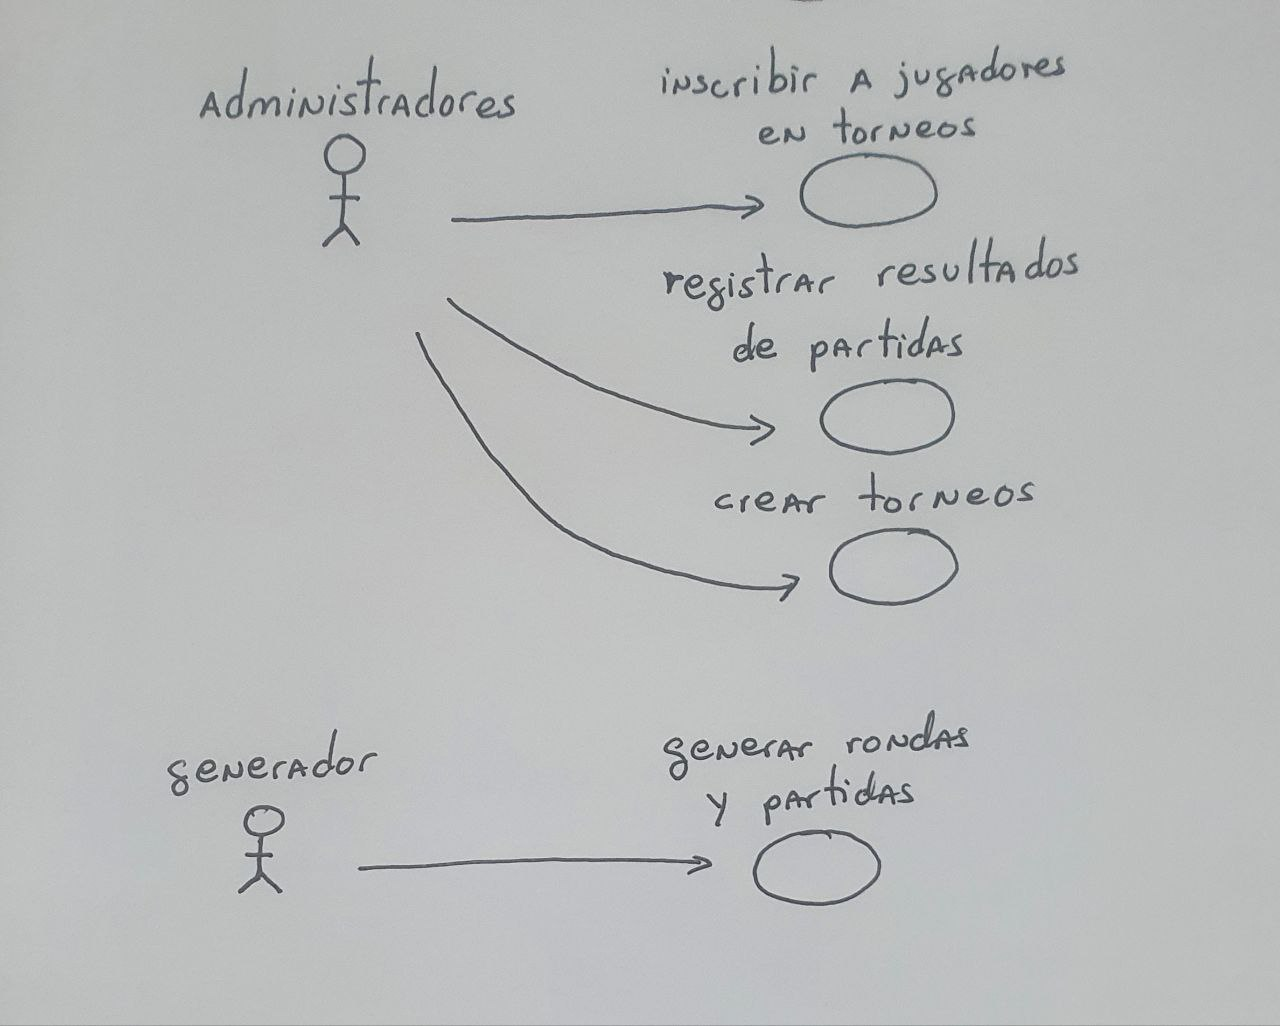
\includegraphics[width=0.5\textwidth]{r2.jpg} 
  		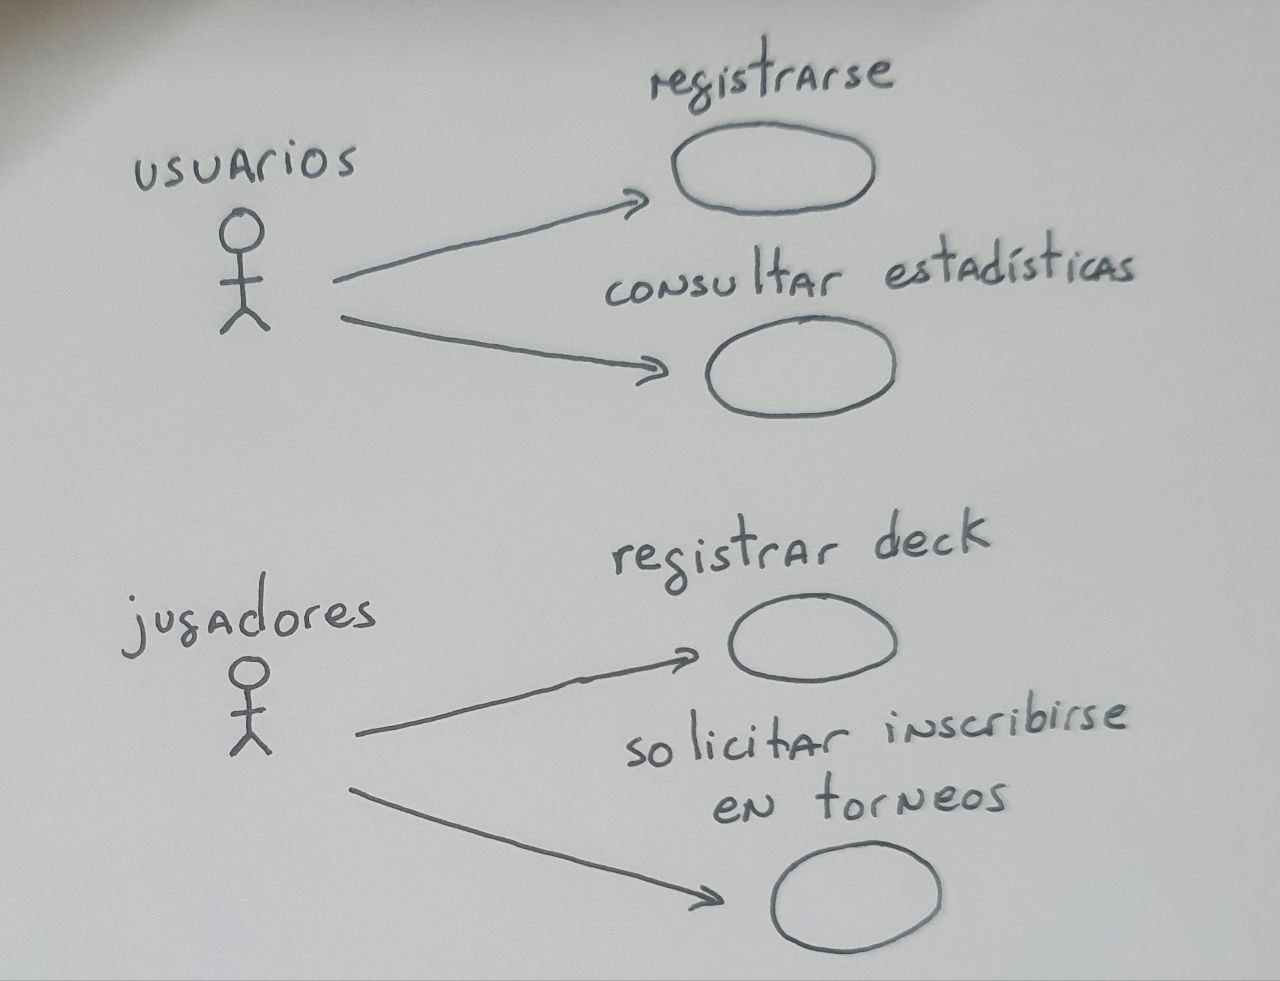
\includegraphics[width=0.5\textwidth]{r3.jpg}  
	\end{figure}
	\begin{figure}[h]  
  		\centering
  		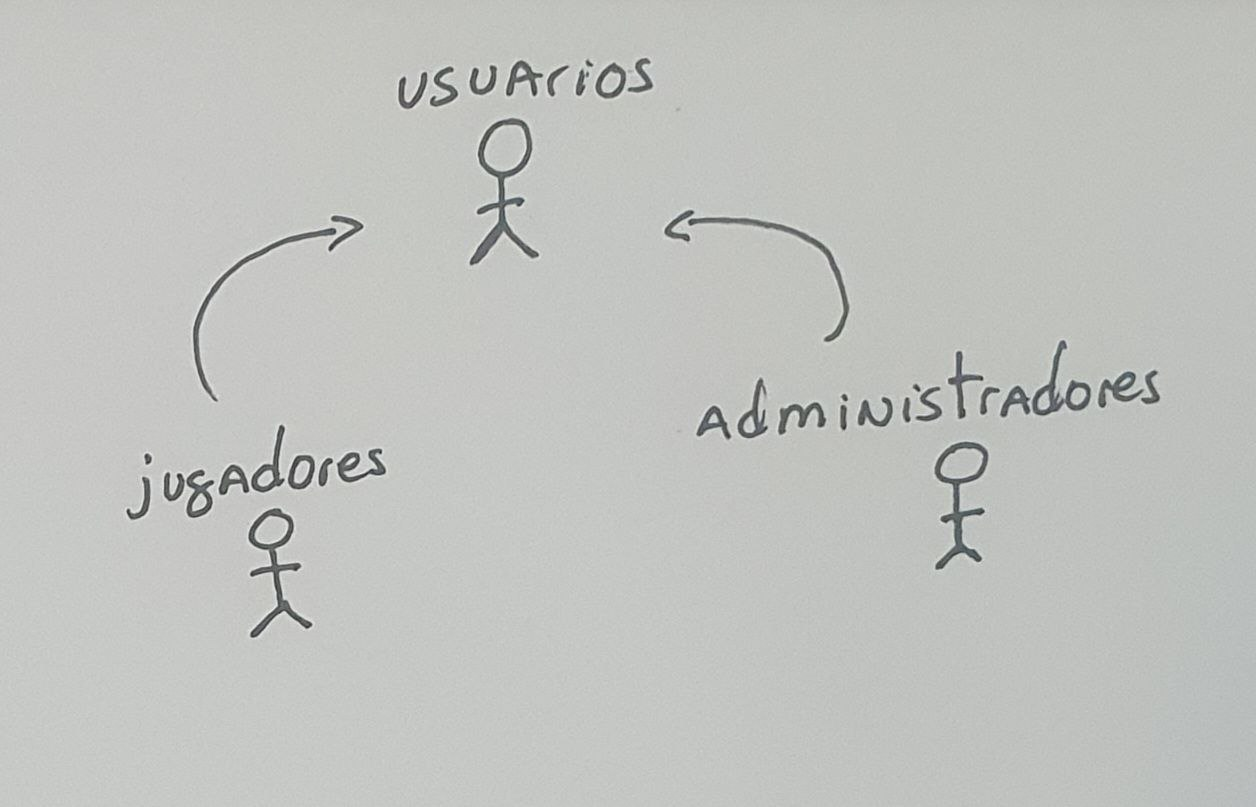
\includegraphics[width=0.5\textwidth]{r1.jpg}
	\end{figure}
\newpage
\section{Enfoque Metodol\'ogico}
Para el proyecto de gestión de torneos de Yu-Gi-Oh!, en el que debes almacenar y analizar información generada a partir de los torneos y facilitar el cálculo de estadísticas de los jugadores, consideramos el uso de la metodología Scrum.
Scrum es un marco de trabajo ágil que se centra en la colaboración, la transparencia y la adaptabilidad, y es particularmente útil para proyectos en los que los requisitos y las prioridades pueden cambiar con el tiempo. Aquí hay algunas razones por las cuales creemos que Scrum es adecuado para este proyecto:
\begin{enumerate}
\item Flexibilidad para cambios: Dado que el proyecto involucra la creación de una base de datos y una aplicación que deben ser adaptables a las necesidades cambiantes de los torneos de Yu-Gi-Oh!, Scrum permite la incorporación de cambios de manera eficiente a través de iteraciones regulares.
\item Colaboración: Scrum fomenta la colaboración estrecha entre los miembros del equipo de desarrollo y los interesados, como los administradores de torneos y los jugadores. Esto es esencial para garantizar que la aplicación se ajuste a las necesidades de los usuarios.
\item Entrega incremental: Scrum divide el trabajo en iteraciones cortas llamadas "sprints". Al final de cada sprint, se tiene una versión funcional de la aplicación que puede ser evaluada por los interesados. Esto permite un desarrollo incremental y la entrega continua de valor.
\item Priorización de características: Scrum utiliza una lista priorizada de características o elementos del producto (el "backlog del producto"). Esto permite que los administradores de torneos y los jugadores prioricen las características más importantes a medida que se desarrollan.
\item Transparencia y visibilidad: Scrum fomenta la transparencia en el proceso de desarrollo, lo que significa que todos los interesados pueden ver el progreso y el estado del proyecto en todo momento.
\item Adaptación continua: Scrum ofrece la capacidad de adaptarse a los cambios en los requisitos y prioridades a medida que surgen. Los equipos Scrum realizan reuniones regulares de revisión y retrospectiva para mejorar el proceso constantemente.
\newpage
\section{Arquitectura}
Hemos optado por la Arquitectura Onion, presentada por Jeffrey Palermo, debido a
su sólido historial de éxito en proyectos de software. Esta elección se basa en los
siguientes motivos clave:
\begin{enumerate}
\item Principio de Inversión de Dependencias: La Arquitectura Onion se adhiere al
Principio de Inversión de Dependencias, promoviendo la independencia entre
capas y la flexibilidad del sistema.
\item Modularidad y Separación de Responsabilidades: Nos permite mantener una
estructura modular y una clara separación de responsabilidades, esenciales
para el desarrollo y mantenimiento eficaz.
\item Testabilidad: Facilita pruebas efectivas, garantizando la calidad y confiabilidad
del código en nuestro proyecto.
\item Flexibilidad y Adaptabilidad: Nos permite adaptarnos a cambios futuros y
nuevas tecnologías sin afectar significativamente la funcionalidad existente.
\item Colaboración Efectiva: Con múltiples ingenieros trabajando en el proyecto, la
Arquitectura Onion establece contratos claros entre capas y componentes, lo
que facilita la colaboración.
\end{enumerate}
\subsection{Capas Externas (Outer Layers)}
\textbf{Infrastructure:} En esta capa reside nuestra base de datos, sistema de archivos o
cualquier servicio web externo del que dependamos.\\
\textbf{Tests:} En esta capa residen pruebas unitarias, de integración y de extremo a
extremo esenciales para garantizar la calidad y la confiabilidad del código.\\
\textbf{User Interface:} Es la capa más cercana a la interfaz de usuario y proporciona una
forma de comunicarse con el núcleo de la aplicación. Esta capa interactúa con la
primera capa del "application core"(application services layer).
\subsection{Núcleo de la Aplicación (Application Core)}
\textbf{Application Services (Transport Layer):} Dentro de esta capa, definimos lo que
nuestro servicio puede hacer a través de una serie de contratos.\\
\textbf{Domain Services:} En esta capa es donde reside la mayor parte de nuestra lógica
de negocios. Lleva a cabo las operaciones para convertir A en B, entrada en salida.
Específicamente en nuestro proyecto, esta capa se encargará de aspectos como la
gestión de emparejamientos, el control de estadísticas, el manejo de algunas reglas
del torneo, la gestión de resultados, el control de decks, entre otros.\\
\textbf{Domain Model:} Es la capa de representación de los objetos de datos de alto nivel
que utilizamos. Aquí se definen y encapsulan los conceptos fundamentales y los
elementos clave del juego, lo que permite una representación fiel y coherente de los
datos en la aplicación. Algunos de los aspectos esenciales que se manejan en esta
capa incluyen la representación de entidades o conceptos fundamentales de la
lógica del proyecto, como jugadores, decks, mazos, partidas y torneos.
\end{enumerate}
\newpage
\section{Patrones de visualizaci\'on y de datos}
En la aplicación de gestión de torneos de Yu-Gi-Oh!, hemos optado por utilizar el enfoque MVC (Modelo-Vista-Controlador) debido a su afinidad con nuestra solución para el mundo del Duelo de Cartas. Este enfoque permite que avancemos en cada componente sin perturbar a los otros, lo que organiza eficazmente el trabajo del equipo.

El $"$Modelo$"$ se encuentra definido por la capa de datos y la implementación de las entidades que representan los usuarios, los mazos de los jugadores, los torneos, y m\'as utilizando Entity Framework (los detalles específicos se discutirán en la sección sobre el patrón de acceso a datos). Para el apartado visual, hemos decidido aprovechar el framework de desarrollo de aplicaciones web React, que se integra de manera efectiva con la tecnología utilizada en el "Controlador." Este último se implementa en C$\#$ con un servidor de ASP.NET, gestionando las solicitudes del apartado visual y estableciendo la conexión con el "Modelo."

Con respecto a los "Patrones de Diseño de Acceso a Datos," hemos elegido el ORM (Mapeo Objeto-Relacional) debido a que estamos trabajando con una base de datos relacional, lo que simplifica la interacción. Utilizamos Entity Framework para aplicar esta estrategia, ya que no estamos limitados por plataformas ni bases de datos específicas. Entity Framework proporciona la comodidad de las consultas LINQ como un medio de interacción. Dado que las consultas SQL que debemos realizar no son particularmente complejas, no anticipamos problemas significativos de rendimiento.

Esta estructura nos permite manejar de manera eficiente la gestión de mazos, torneos y partidas en la aplicación, lo que es esencial para la organización de eventos de Yu-Gi-Oh!. Además, la aplicación será capaz de responder a una serie de consultas y análisis de datos para brindar información relevante a los Duelistas
\newpage
\section{Modelo de datos}
	\begin{figure}[h]
  		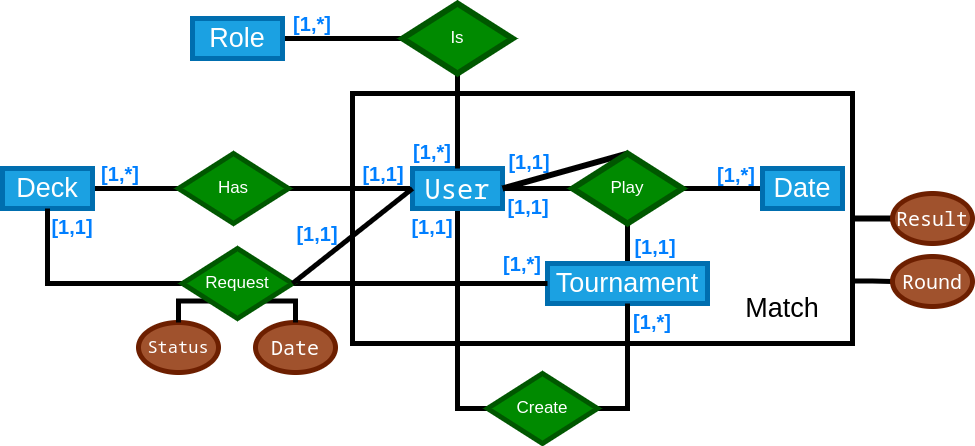
\includegraphics[width=1\textwidth]{merx.png} 
	\end{figure}
\newpage
\section{Diccionario De Datos}
	\begin{figure}[h]
  		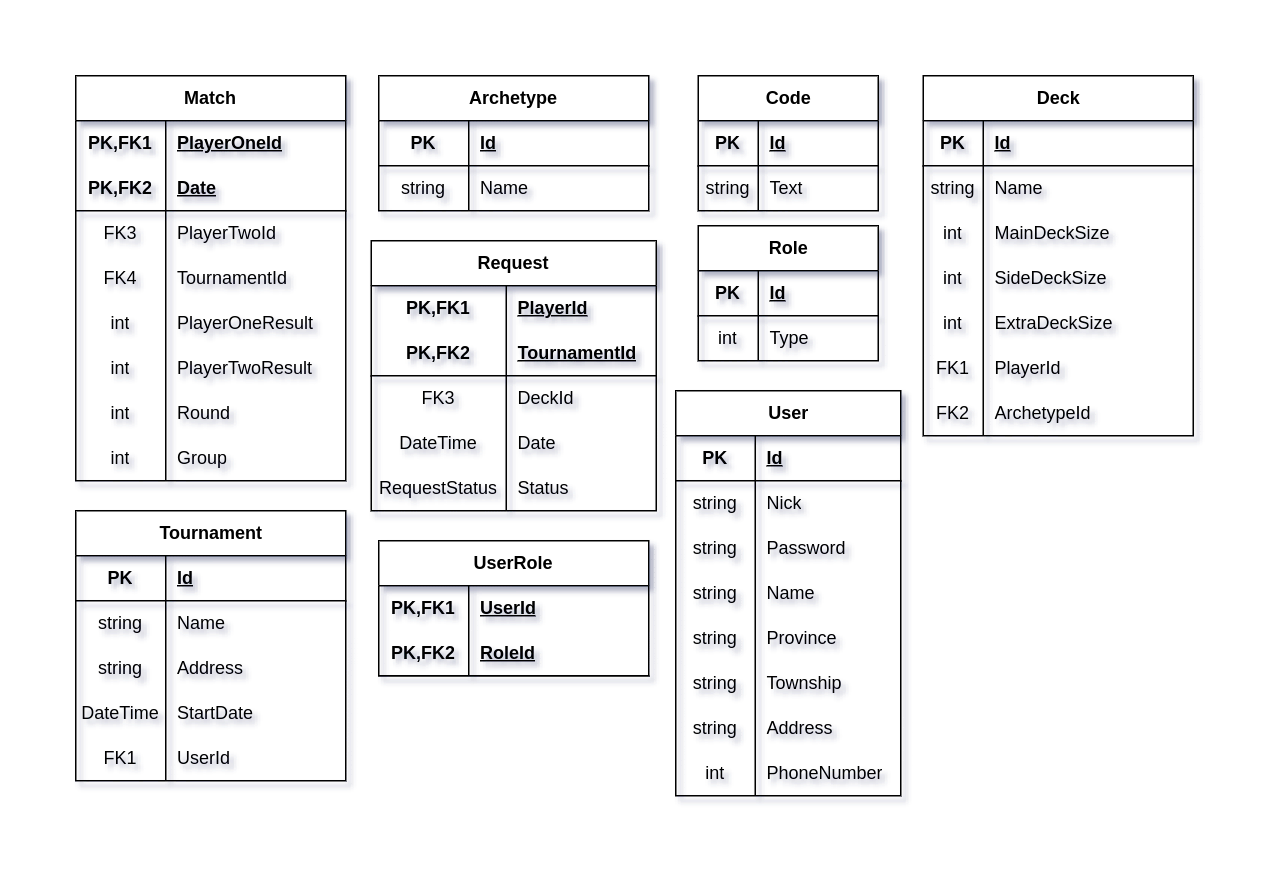
\includegraphics[width=1\textwidth]{dic.png} 
	\end{figure}
	
\newpage
\section{Esquema de clases definidas}
	\begin{figure}[h]
  		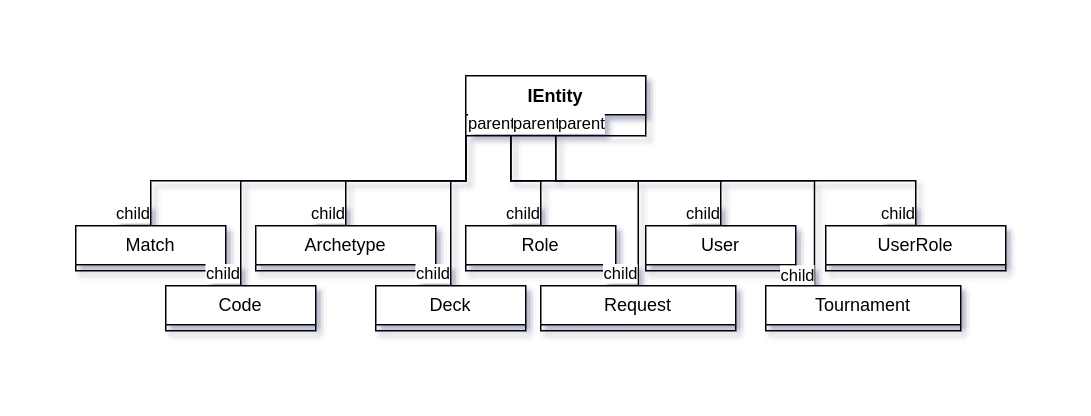
\includegraphics[width=1\textwidth]{ClasesDefinidas.png} 
	\end{figure}
	\begin{figure}[h]
  		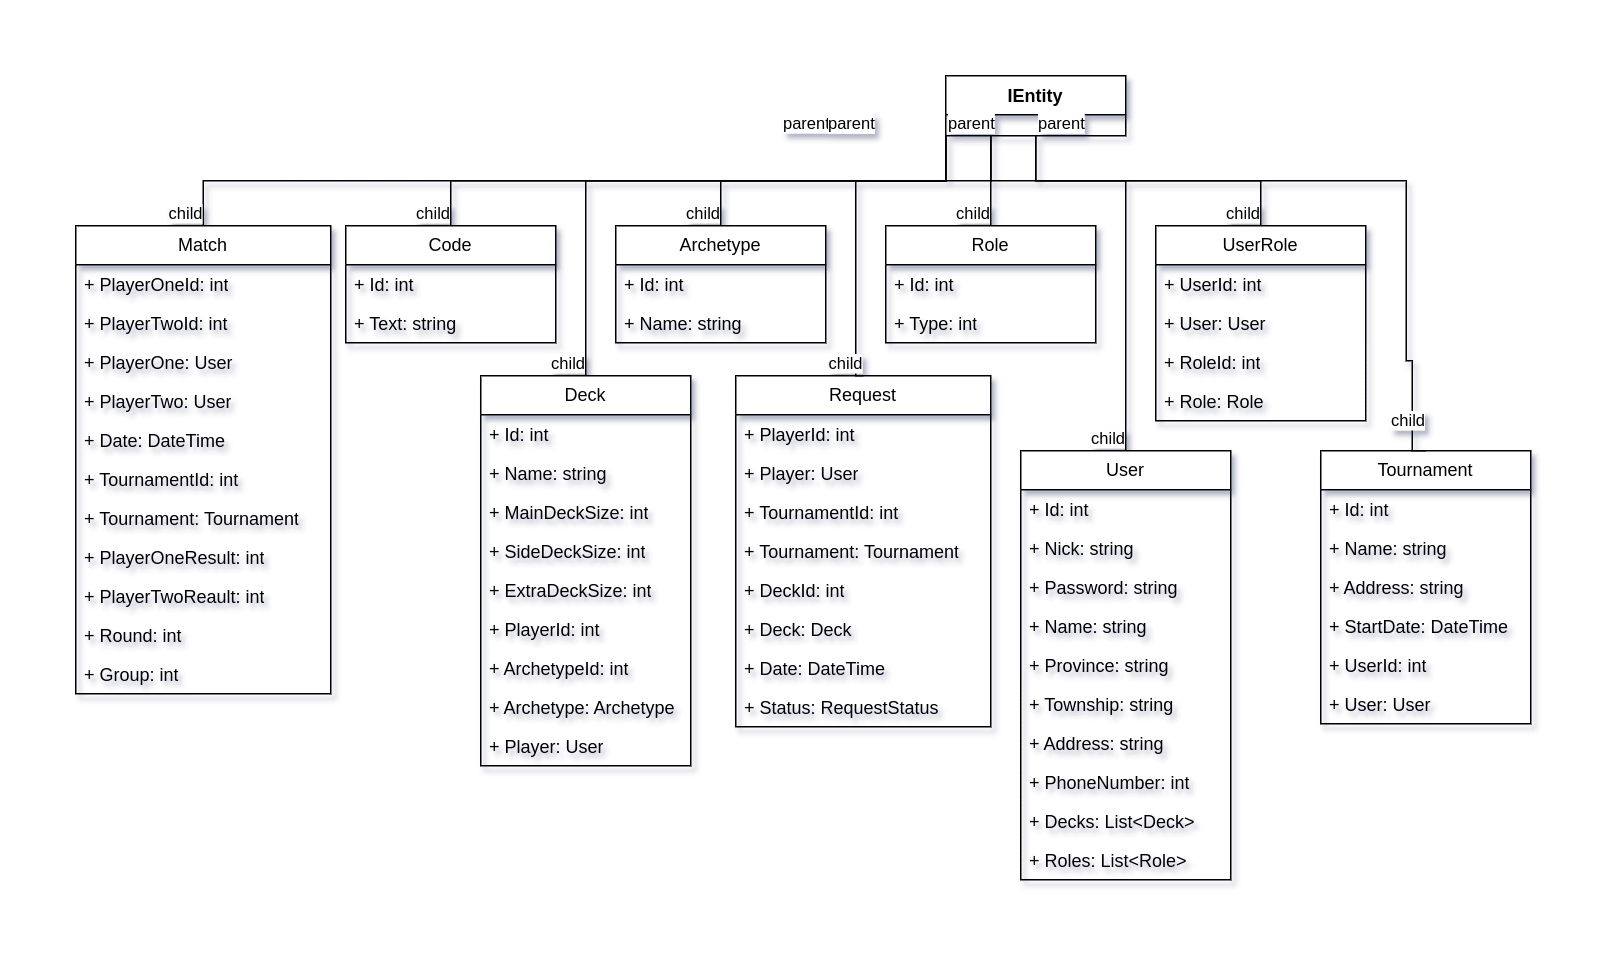
\includegraphics[width=1\textwidth]{ClasesDefinidasExtendido.png} 
	\end{figure}


\end{document}
